% !TEX root = ../main.tex
%--- Slide 7: la degenerazione non dipende dal modello (circa 50 s) ----------------------
% Figura: Figure/P07_reali_8par_BN_DM.pdf (notebook 26) = Fig. 5.3 della tesi ridotta a band noise e DM.
\begin{frame}{La degenerazione resta con modelli più complessi}
  \begin{columns}[c]
    \column{0.52\textwidth}\small
    \textbf{Band noise nel modello} (8 parametri)
    \begin{itemize}\setlength{\itemsep}{1pt}
      \item Rumore rosso solo sui TOA della banda LOFAR
      \item Non rivelato: solo un limite superiore
            $\log_{10}A_{\rm BN} < -12.21$ (95\%)
      \item Il DM ha ancora due picchi
    \end{itemize}
    \vspace{2mm}
    \textbf{Indice cromatico $\alpha$ libero} (7 parametri)
    \begin{itemize}\setlength{\itemsep}{1pt}
      \item $\alpha = 3.31^{+0.60}_{-0.46}$
      \item Due picchi e contorni a L restano
    \end{itemize}
    \vspace{3mm}
    \fbox{\parbox{0.92\linewidth}{\centering
      La degenerazione non è dovuta a un modello impreciso dello scattering}}
    \column{0.46\textwidth}
    \centering
    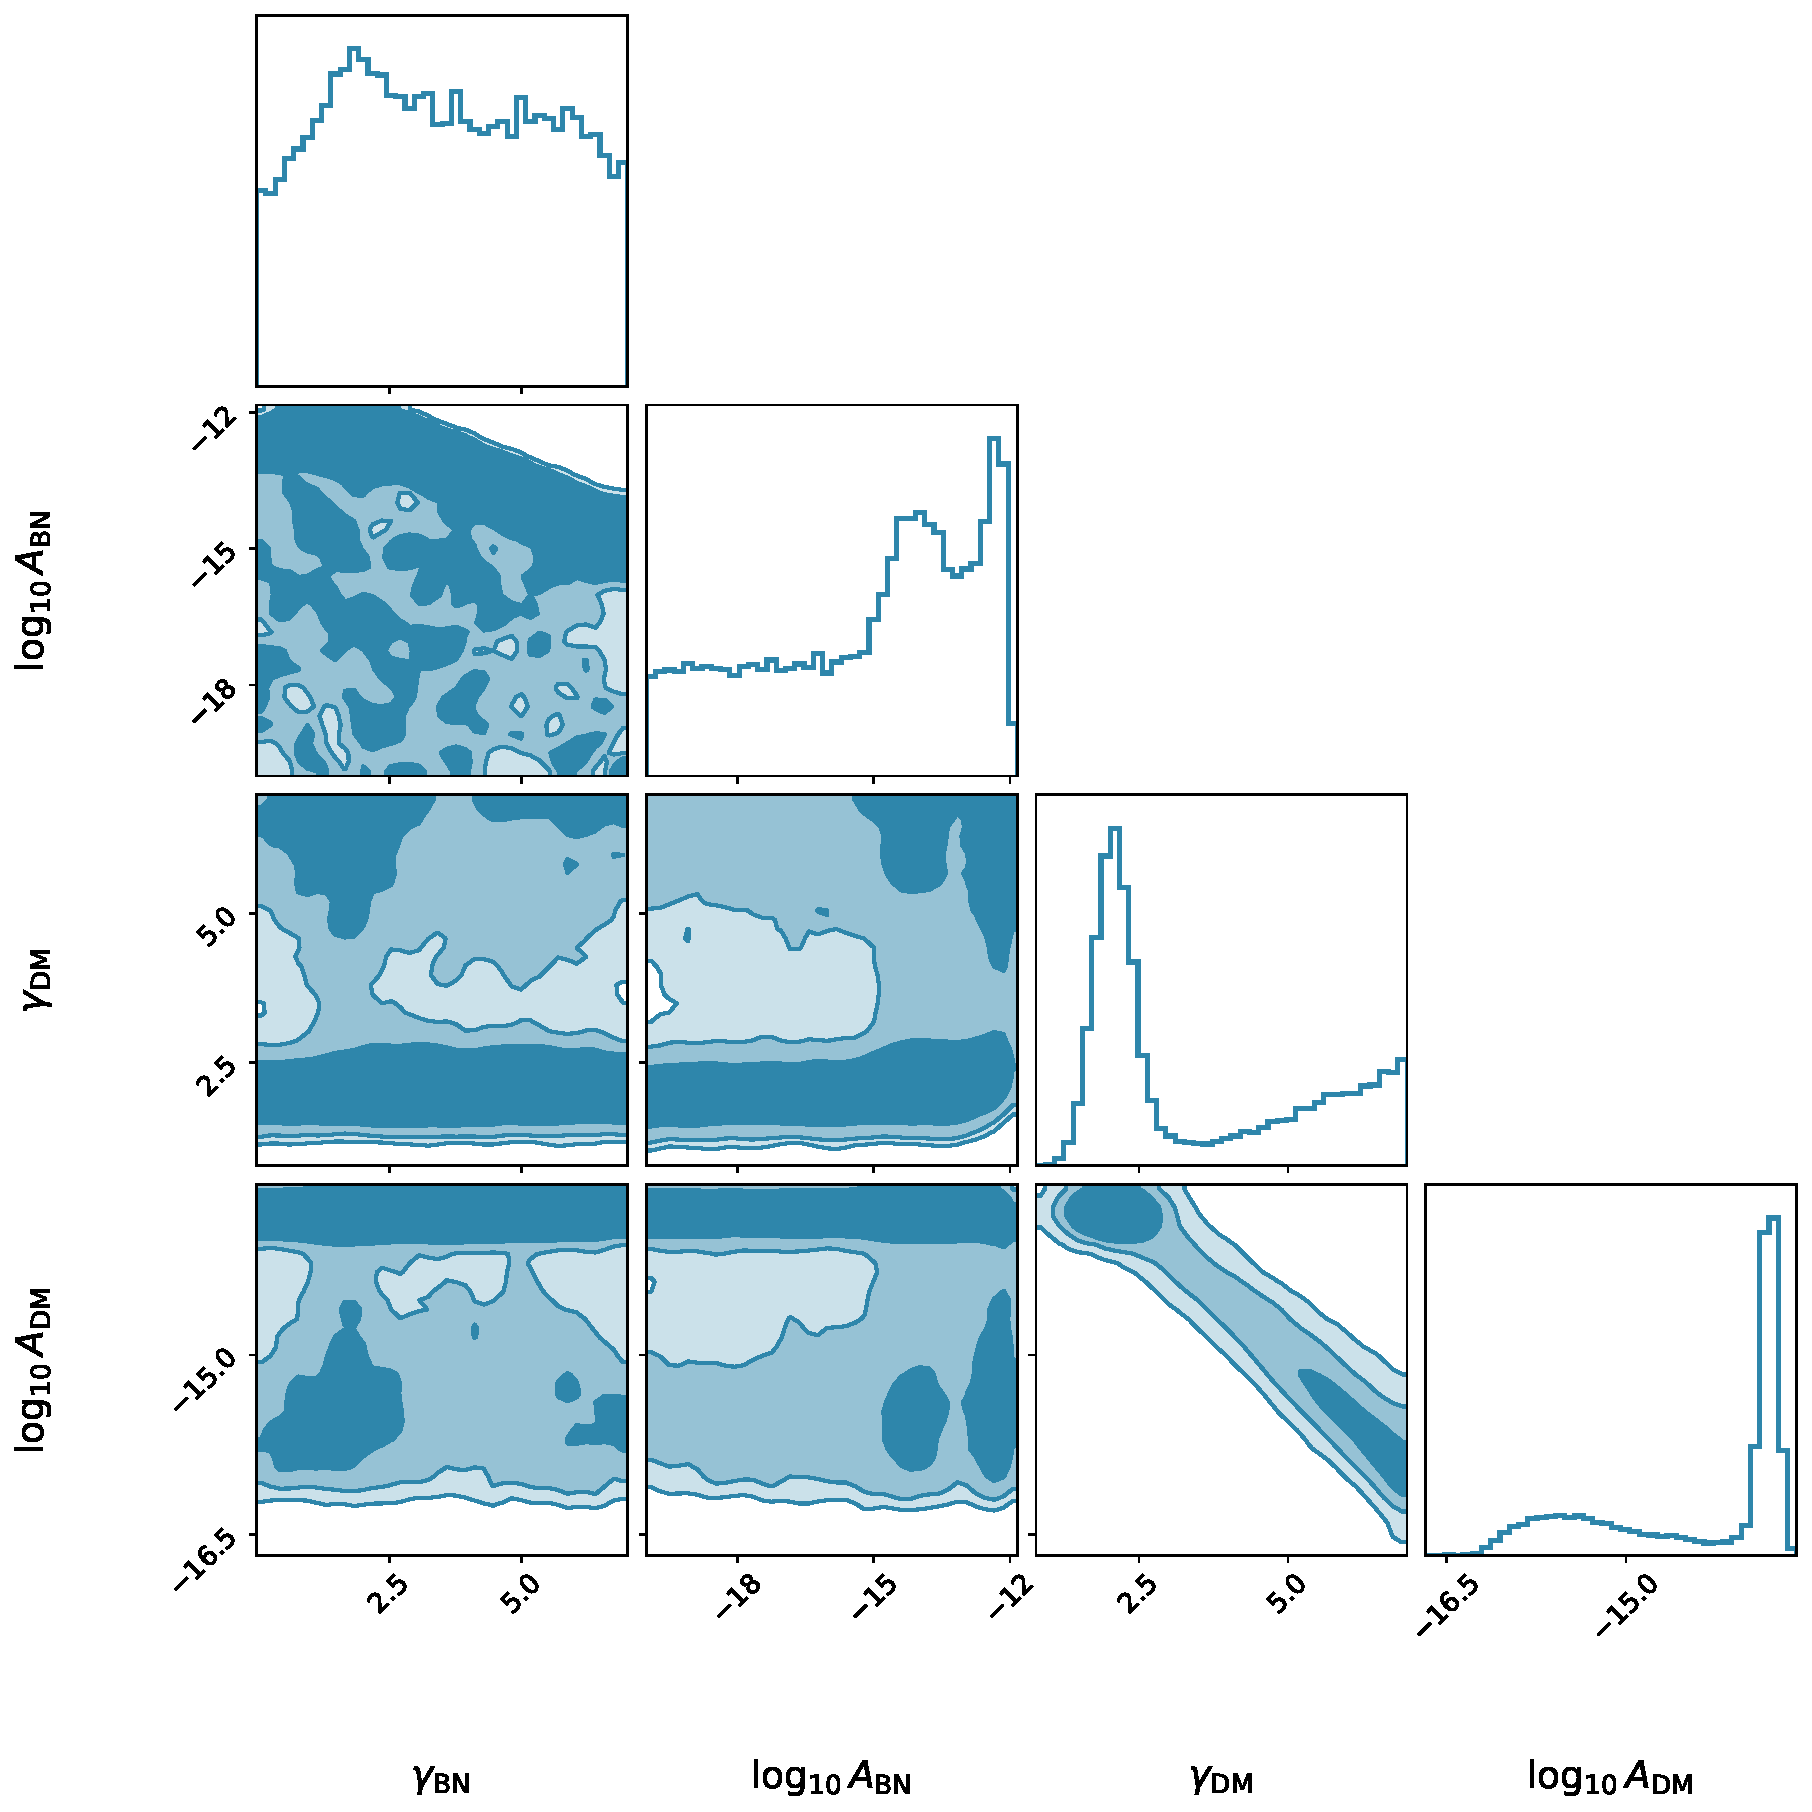
\includegraphics[height=0.72\textheight]{Figure/P07_reali_8par_BN_DM.pdf}\par
    {\footnotesize \reali{dati reali}, modello con band noise}
  \end{columns}
\end{frame}
